% This file is isea.tex.  It contains the formatting instructions for and acts as a template for submissions to ISEA 2015.  It is based on the ICCC  formats and instructions.  It uses the files isea.sty, isea.bst and isea.bib, the first two of which also borrow from AAAI IJCAI formats and instructions.
% Modified from ICCC.tex by B. Bogart

\documentclass[letterpaper]{article}
\usepackage{isea}
\usepackage{amsmath,amssymb,amsfonts}
\usepackage{algorithmic}
\usepackage[pdftex]{graphicx}
\usepackage{times}
\usepackage{helvet}
\usepackage{courier}
\usepackage{xcolor}
\usepackage{minted}
\usepackage{caption}
\usepackage[numbers]{natbib}
\usepackage[export]{adjustbox}
\graphicspath{ {./images/} }
\pdfinfo{
/Title (Test Your Limits With TRex Traffic Generator)
/Author (Hanoch Haim)}
% The file isea.sty is the style file for ISEA 2015 proceedings.
%
\title{Test Your Limits With TRex Traffic Generator}
\author{Hanoch Haim, 
Cisco Systems \\
\newline
\newline
}
\setcounter{secnumdepth}{0}


\begin{document} 
\maketitle
\begin{abstract}
Performance measurement tools are an integral part of network testing. 
There is no shortage of open source tools for network performance
testing in the Linux world. 
To enumerate a few popular tools in the Linux world: Netperf, iperf, Linux kernel based pktgen.
These tools tend to fall into two categories:
\begin{itemize}
\item Stateless packet shooting such as the Linux kernel pktgen traffic generator 
\item Stateful client-server tools such as netperf and iperf. 
\end{itemize}  
When very high performance network performance testing is required (quantified as
many 10s of Gigabits per second/100MPPS and/or hundreds of thousands of flows) or more advanced functionality (e.g. realistic) is required the
Linux classical tools are insufficient. Most organizations
will opt for very expensive commercial tools such as Ixia, Spirent. 
In this paper we will introduce TRex a high performance realistic traffic generator
and illustrate sample stateless and stateful use cases that apply to testing
Linux networking. We will also discuss its design and tricks that help us
achieve such high performance.
\end{abstract}
    
\section{Keywords}

tcp, performance, scale,realistic traffic generation 

\section{Introduction}

TRex \cite{b1} is an advanced traffic generator, it has the following interesting features:

\begin{itemize}
\item It leverages COTS x86/ARM servers and physical NICs (Intel, Mellanox etc) for high scale.
\item Can support Linux driver or virtual (e.g. virtio/veth) for low scale with advanced features \texttt{(PF\_PACKET)}
\item It can serve both stateless and stateful traffic generation.
tcp stack for stateful traffic and emulation layer to simulate L7 applications.
\item It outperforms all of iperf, netperf and kernel pktgen: 
\begin{itemize}
    \item It can generate upto 200gbps/100mpps advance complex patterns and millions of real
    world tcp/udp flows.
    \item High connection rate - order of Millions of Connection/s (CPS).
\end{itemize}
\item It is extensible:
\begin{itemize}
    \item Can emulate L7 application (on top of TCP/IP),
    e.g. HTTP/HTTPS/Citrix using a DSL programmable language described in Python 
    \item Ability to change fields in the L7 application - for example,
    change HTTP User-Agent field
\end{itemize}
\item Support routing protocols like BGP/OSPF/RIP using BIRD \cite{b4}
\item Support high scale clients simulation protocols like arp,ipv6-nd,dhcp4,dhcp6,802.1x,icmp,igmp,mld using a new process written in golang 
\end{itemize}
Although TRex is implemented on top of DPDK, a lot of the issues we had
to deal with when writing the tool apply equally to scaling Linux networking;
we share our experiences in that regard and hope to inspire some
of the techniques to be adopted in Linux.

\section{Software design high level}

\begin{figure}[h]
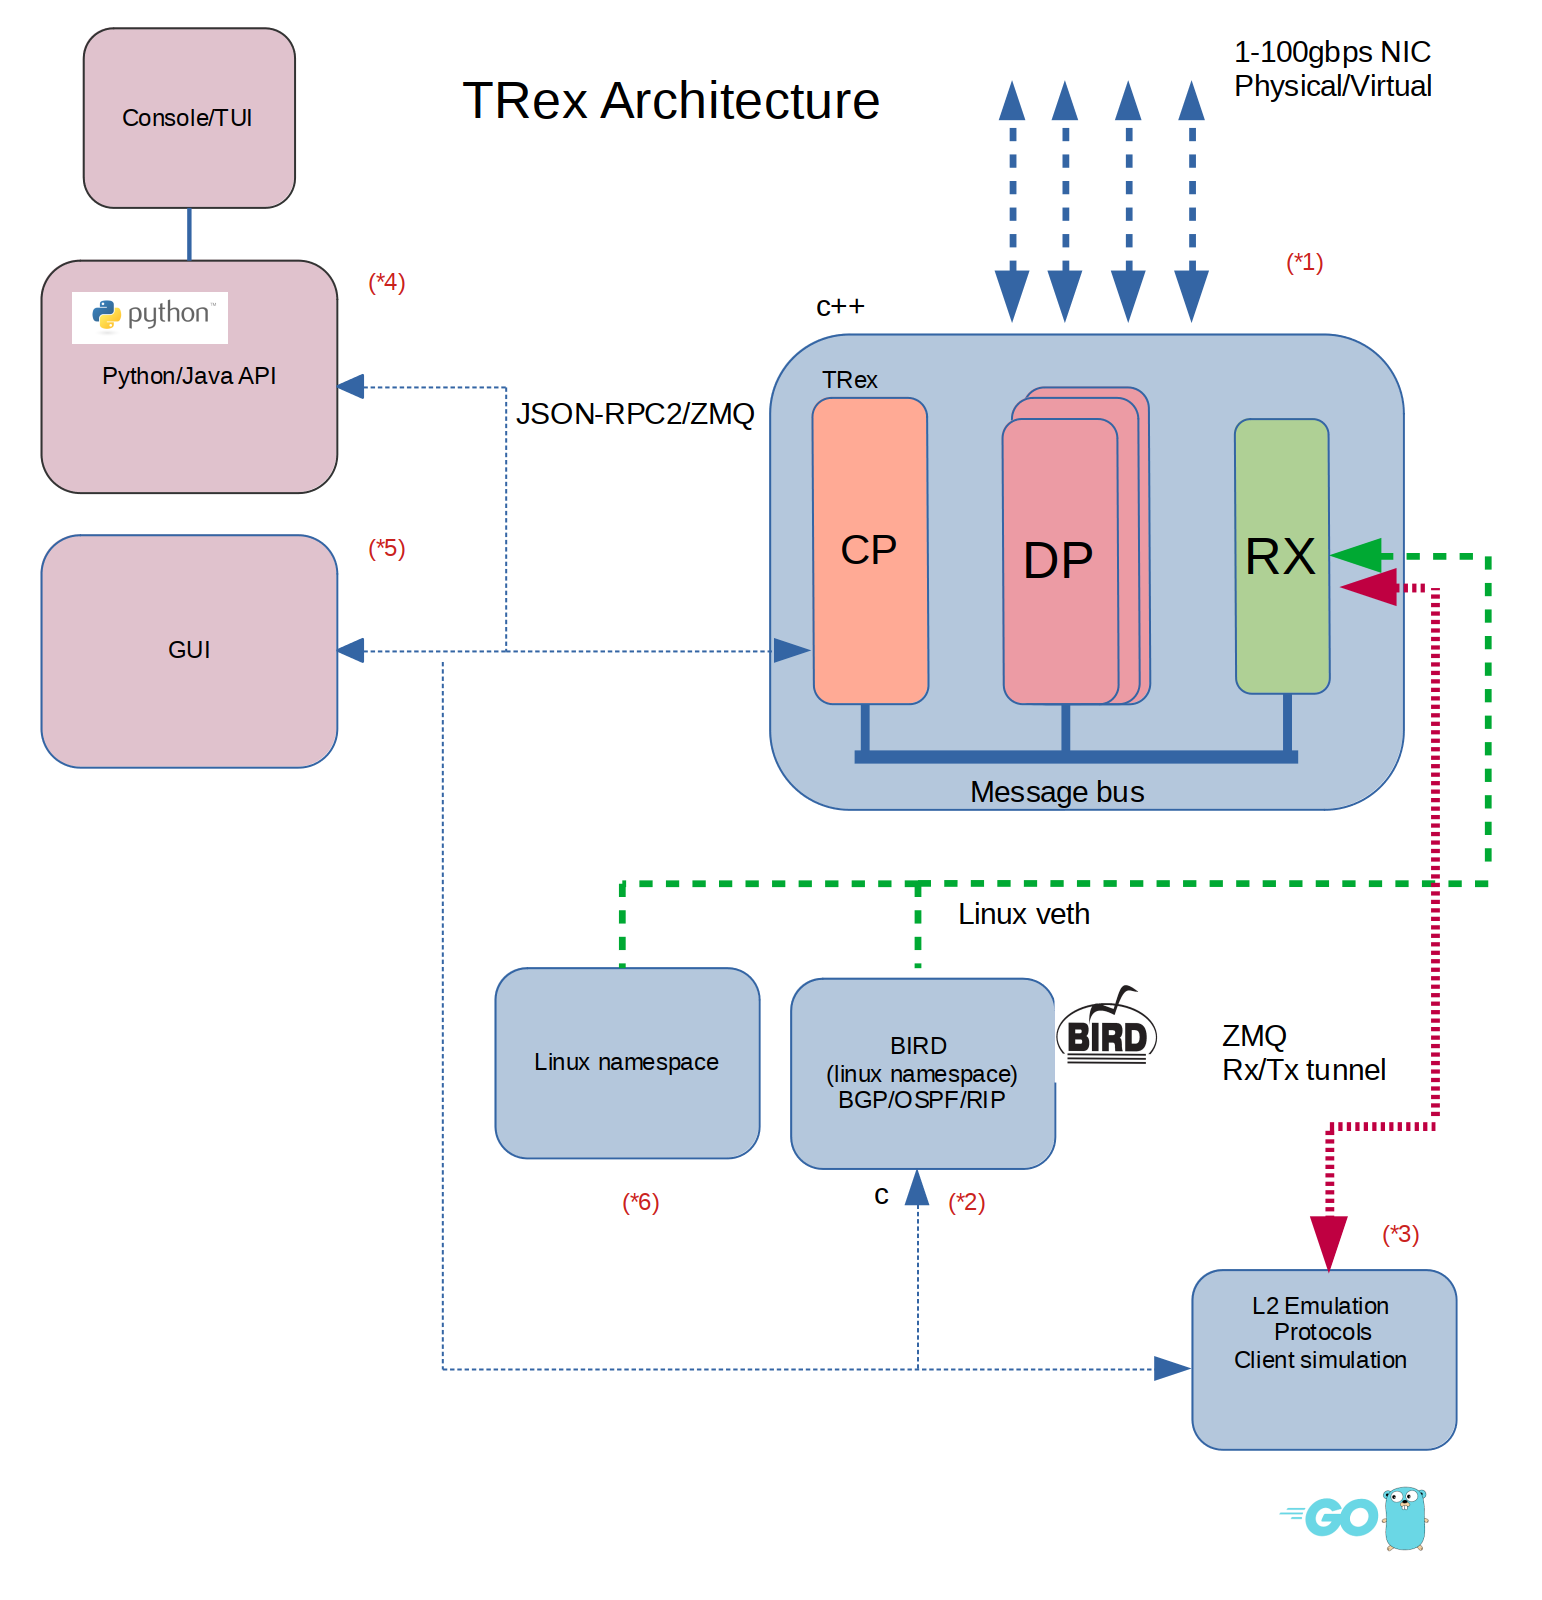
\includegraphics[width=0.4
\textwidth, center]{trex_arch_2.png}
\caption{Architecture}
\label{fig:arch}
\end{figure}

Figure \ref{fig:arch} presents the main processes. TRex server (*1) is a multi-threaded process, each thread is pinned to a core and works in 
event driven fashion using a user-space scheduler with a few levels of hierarchy. There is one control-plane (CP) thread that handles the RPC over ZMQ requests and maintenance tasks. 
The RX thread is responsible for accurate latency measurement. This thread usually consumes very low CPU utilization. 
The DP threads generate the traffic using DPDK to transmit/receive traffic via PMD queues. 
The number of DP threads can be scaled up to the number of available Tx/Rx queues. 
There is almost no memory sharing data structure and no locks to achieve the best performance. 
Almost all the information between the threads is exchanged using a messaging bus which 
is composed of shared rings (DP$\rightarrow$CP, CP$\rightarrow$DP, Rx$\rightarrow$DP, Rx$\rightarrow$CP).
The system calls to the kernel are kept at minimum(only when required for example with PF\_PACKET/AF\_XDP driver)
(*4) is a Python wrapper to the JSON-RPC2 API over ZMQ to supply easy automation (e.g. load a profile, get statistics etc).
On top of Python API there is a Console that can simplify the way to work with the API. 
(*5) is the GUI written in Java that works directly with the JSON-RPC2 and supports only the stateless mode.
(*2) is a BIRD \cite{b4} process that works inside a Linux namespace and connects to TRex via a programmable veths. Inside TRex's RX thread there is a Switch that forwards packets to/from the veth related to the Linux namespace. 
BIRD is used to simulate routing protocols like BGP/OSPF/RIP.
(*6) and (*3) is used for simulating clients slow-path protocols like ARP/IPV6-ND/IGMP/MLD/802.1x/DHCP/DHCPv6 while TRex server is for the fast-path high speed TCP/UDP

\subsection{Dataplane scheduler}

\begin{figure}[h]
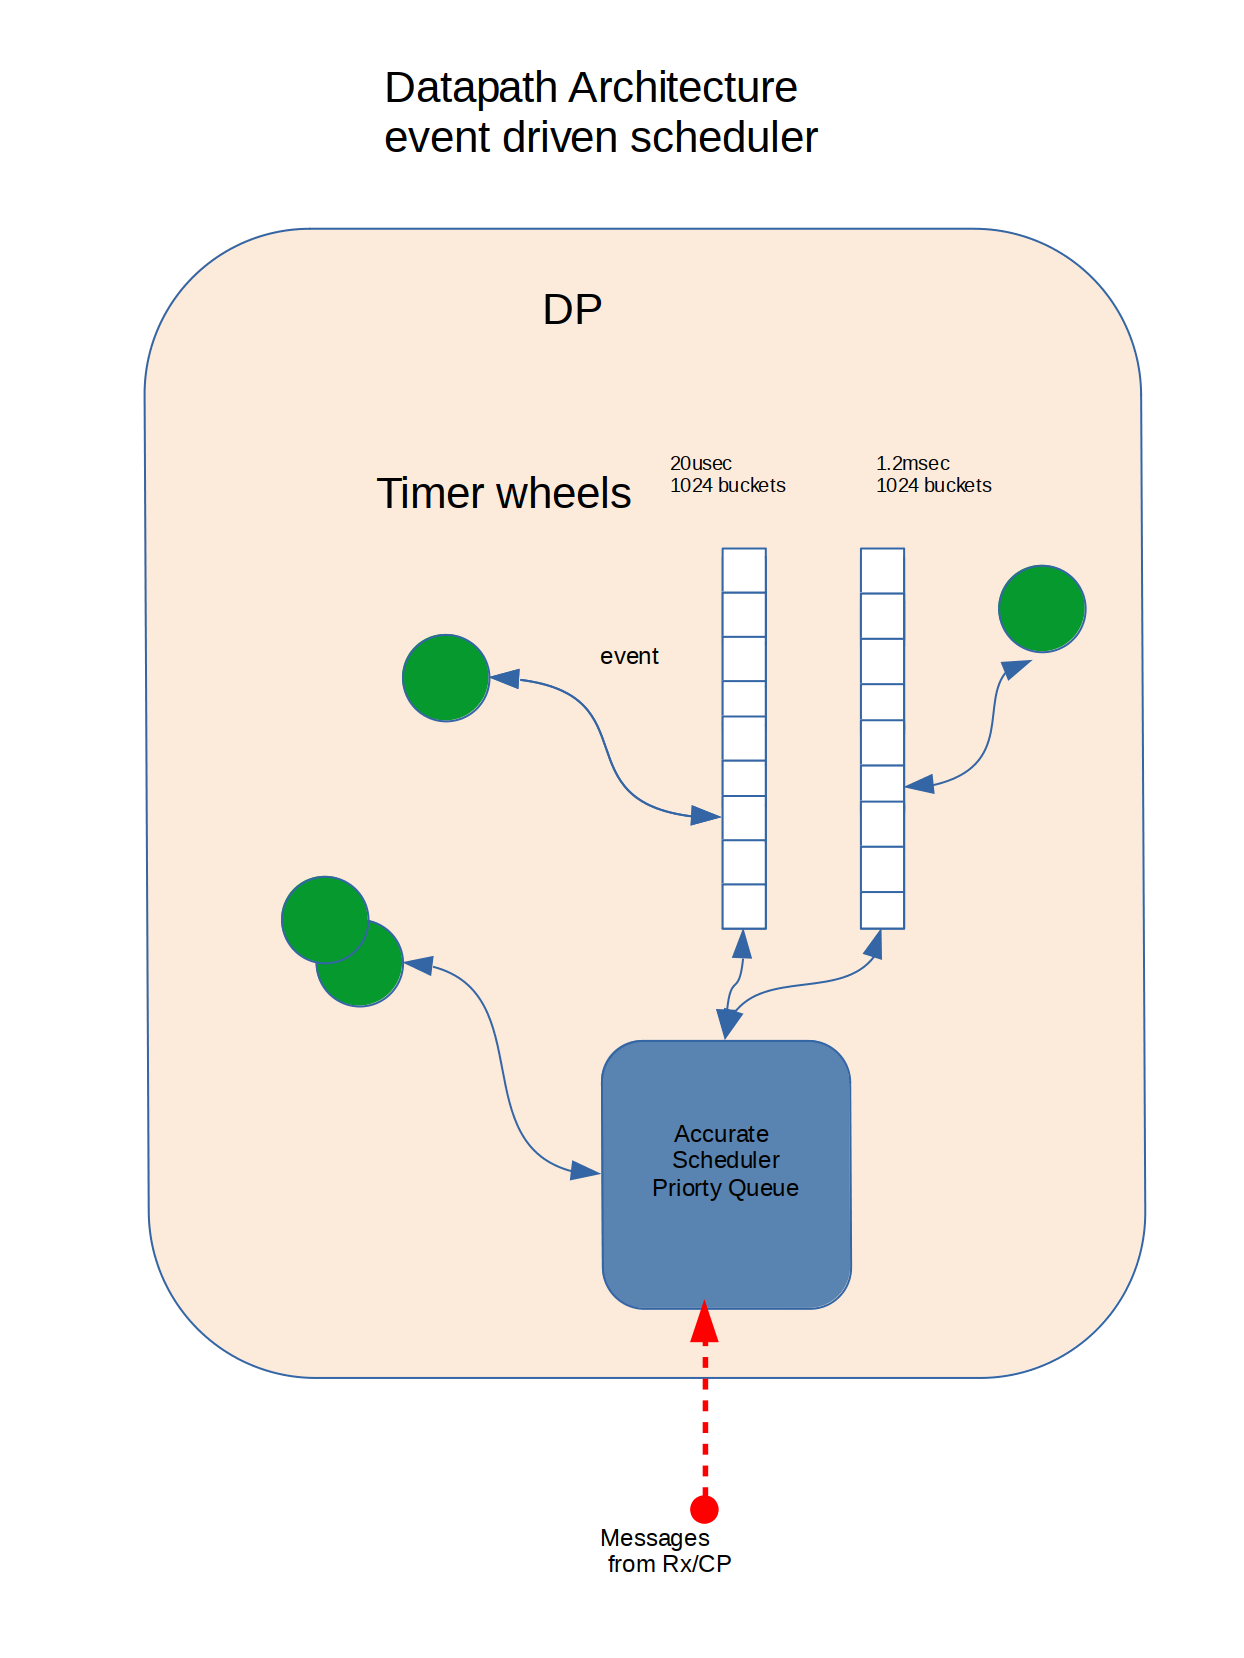
\includegraphics[width=0.3
\textwidth, center]{trex_dp_sheduler.png}
\caption{Dataplane Scheduler}
\label{fig:dp_schduler}
\end{figure}
  
Figure \ref{fig:dp_schduler} presents the schedulers in each DP thread. The priority queue is the low level scheduler that can schedule events at nsec resolution. In addition there are two timer wheels for lower resolution events. The first timer wheel has a resolution of 20usec with 1024 buckets for maximum of 2msec time. 
The second timer wheel has resolution of 1msec with 1024 buckets and maximum of 1sec which cover most of the timer duration needed. Each event in the second level is spread each 20usec tick to reduce processing spikes. 
The DPs transmit/receive messages from the shared rings using events. 
This design achieves linear scale with a performance about 4-20MPPS/core and 200gbps for one COGS server. 

\begin{figure}[h]
\includegraphics[width=0.4
\textwidth, center]{sfr_profile.png}
\caption{emix}
\label{fig:emix}
\end{figure}

\subsection{Operation modes}

From the functionality point of view TRex has two main operation modes: stateful and stateless. 

Stateful is meant for testing L7 services that care about clients/flows/L7 application like DPI/NAT/Firewall, Figure \ref{fig:emix} is an example of a mix of traffic that can be generated using this mode. 

Stateless is meant for testing Switch/Filters/ACL/QoS services and has no flow/client state context.

\section{Stateless mode}

Stateless mode is meant to test networking gear/feature that does not manage any state per flow (instead operating on a per packet basis). 
This is usually done by injecting customized packet streams to the device under test.

\begin{figure}[h]
\includegraphics[width=0.25
\textwidth, center]{stateless_objects_02.png}
\caption{Stateless main objects}
\label{fig:stlobjects}
\end{figure}

Figure \ref{fig:stlobjects} shows the model of a profile. Each interface supports one or more traffic profiles in parallel.
Each traffic profile supports one or more streams. Each stream includes the following main properties:

\begin{itemize}
\item \textbf{Packet}: Packet template up to 9 KB
\item \textbf{Field Engine}: A program that determines which field to change and how to change 
\item \textbf{Mode}: Specifies how to send packets \{Continuous, Burst, Multi-burst\}
\item \textbf{Rx Stats}: Which statistics to collect for each stream
\item \textbf{Rate}: Rate (pps or bps) 
\item \textbf{Action}: Specifies stream to follow when the current stream is complete (valid for Continuous or Burst modes)
\end{itemize}

\begin{figure}[h]
\includegraphics[width=0.4
\textwidth, center]{stl_interleaving_01.png}
\caption{Stateless profile example}
\label{fig:stlhello}
\end{figure}

Figure \ref{fig:stlhello} shows an example of a profile with three streams.  
Stream 1 has a rate of 10pps stream 2 has a rate of 20 pps and streams 3 has rate of 40 pps. All are configured for continuous mode.

Listing \ref{listing:1} shows a simplified profile that matches Figure \ref{fig:stlhello}. The mode is Continuous. 
It uses Scapy for building the template packet. This profile is converted to json and sent to the TRex server for processing. 

\begin{listing}[h]
\caption{Profile with one continues UDP stream}
\label{listing:1}
\begin{minted}
[
    frame=lines,
    fontsize=\scriptsize,
]
{python}
class STLS1(object):

def __init__ (self):
    self.fsize  =64; # the size of the packet 

def create_stream (self):

    # Create base packet and pad it to size
    size = self.fsize - 4; # HW will add FCS
    base_pkt =  Ether()/
                IP(src="16.0.0.1",dst="48.0.0.1")/
                UDP(dport=12,sport=1025)
    pad = max(0, size - len(base_pkt)) * 'x'


    return STLProfile( 
    [ STLStream(isg = 1.0, # start in delay in usec 
        packet=STLPktBuilder(pkt=base_pkt/pad),
        mode=STLTXCont(pps=10),
        ), 

        STLStream(isg = 2.0,
        packet= STLPktBuilder(pkt=base_pkt/pad),
        mode= STLTXCont(pps=20),
        ),

        STLStream(isg = 3.0,
        packet = STLPktBuilder(pkt=base_pkt/pad),
        mode = STLTXCont(pps=40))
    ]).get_streams()
\end{minted}
\end{listing}
  
\subsection{Stateless Features}

\begin{itemize}
\item Large scale - Supports about 10-22 million packets per second (mpps) per core, scalable with the number of cores
\item Support for 1, 10, 25, 40, and 100 Gb/sec interfaces with DPDK or PF\_PACKET.
\item Support for multiple stateless traffic profiles per interface each profile supports multiple streams. 
\item Programmable Field Engine to change any field inside the packet template i.e. \mint{html}|src_ip=10.0.0.1 - 10.0.0.255| 
\item Ability to change the packet size 
\item API,Console, GUI
\item Statistics, per interface,per stream 
\item Latency and jitter per stream
\item Multi-user support 
\end{itemize}

\subsection{Multi stream profile example}


Figure \ref{fig:stlmulti} shows two streams. Stream 0 is a burst that activates a multi-burst Stream 1 (With 5 burst of 4 packets). 
Listing \ref{listing:4} shows the Python script to create this profile.

\begin{figure}[h]
\includegraphics[width=0.4
\textwidth, center]{stl_multiple_streams_01.png}
\caption{Multi stream profile}
\label{fig:stlmulti}
\end{figure}


\begin{listing}[h]
\caption{Multi profile example}
\label{listing:4}
\begin{minted}
[
    frame=lines,
    fontsize=\scriptsize,
]
{python}
  
def create_stream (self):

# create a base packet and pad it to size
size = self.fsize - 4 # no FCS
base_pkt =  Ether()/
            IP(src="16.0.0.1",dst="48.0.0.1")/
            UDP(dport=12,sport=1025)
base_pkt1 =  Ether()/
            IP(src="16.0.0.2",dst="48.0.0.1")/
            UDP(dport=12,sport=1025)
pad = max(0, size - len(base_pkt)) * 'x'

return STLProfile( 
[ STLStream( isg = 10.0, # start in delay                                  1
    name    ='S0',
    packet = STLPktBuilder(pkt=base_pkt/pad),
    mode = STLTXSingleBurst(pps=10, 
                            total_pkts=self.burst_size),
    next = 'S1'), # run s1 after s0 

    # stream is disabled. Enabled by S0 
    STLStream( self_start = False, 
    name    ='S1',
    packet  = STLPktBuilder(pkt=base_pkt1/pad),
    mode    = STLTXMultiBurst(pps = 1000,
                                pkts_per_burst = 4,
                                ibg = 1000000.0,
                                count = 5)
                            )
                    ]).get_streams()
\end{minted}
\end{listing}


\subsection{Field Engine}

The field engine (FE) is a programmable engine that can change any field in the packet and is part of the profile and compiled into bytecode in the TRex server. 
The challenge was to provide an engine that can change packet fields on a number of cores in parallel but as a black-box it behaves as if it runs on a single core (hardware like).
FE works on stateless mode only. Let us provide an example of a syn-attack profile with a simple field engine program and explain it:

\begin{listing}[h]
\caption{FE syn-attack on 48.0.0.1 server}
\label{listing:2}
\begin{minted}
[
    frame=lines,
    fontsize=\scriptsize,
]
{python}
class STLS1(object):
""" attack 48.0.0.1 at port 80
"""
def create_stream (self):

    # TCP SYN
    base_pkt  = Ether()/
                IP(dst="48.0.0.1")/
                TCP(dport=80,flags="S")

    # create an empty program (VM)
    vm = STLVM()

    # define two vars
    vm.var(name = "ip_src", 
            min_value = "16.0.0.0", 
            max_value = "18.0.0.254", 
            size = 4, 
            op = "random")
      
    vm.var(name = "src_port", 
            min_value = 1025, 
            max_value = 65000, 
            size = 2, 
            op = "random")
        
    # write src IP and fix checksum
    vm.write(fv_name = "ip_src", 
            pkt_offset = "IP.src")
      
    vm.fix_chksum()
        
    # write TCP source port
    vm.write(fv_name = "src_port", 
            pkt_offset = "TCP.sport")
        
    # create the packet
    pkt = STLPktBuilder(pkt = base_pkt, vm = vm)

    return STLStream(packet = pkt,
                    random_seed = 0x1234,
                    mode = STLTXCont())
\end{minted}
\end{listing}
  
Listing \ref{listing:2} shows a FE program that generates a syn-attack using one stream. 
Each stream object has a context for FE variables. In this example there are two variables,
\texttt{ip\_src} for the range of the source IPv4 ips and the \texttt{source\_port} for the range of the source tcp ports.
Those variables are written to the right offset in the packet and the checksum is fixed accordingly (using hardware assist if possible).

\subsection{Automation using Python API}

Listing \ref{listing:6} shows a simple script to automate TRex. It is self-explanatory.

\begin{listing}[h]
\caption{Stateless automation example}
\label{listing:6}
\begin{minted}
[
    frame=lines,
    fontsize=\scriptsize,
]
{python}
 
c = STLClient(username="itay",
            server = "10.0.0.10", 
            verbose_level = "error")
try:
    # connect to server
    c.connect()

    # prepare our ports 
    c.reset(ports = [0, 1])

    # add both streams to ports
    c.add_streams(s1, ports = [0])

    # clear the stats before injecting
    c.clear_stats()

    c.start(ports = [0, 1], 
            mult = "5mpps", 
            duration = 10)

    # block until done
    c.wait_on_traffic(ports = [0, 1])

    # check for any warnings
    if c.get_warnings():
    # handle warnings here
    pass

finally:
    c.disconnect()
\end{minted}
\end{listing}
 
\subsection{Stateless Performance}

Figure \ref{fig:stlperf} \cite{b5} shows the measured performance on a Cisco UCS server with dual socket CPU E5-2667 v3@3.20GHz 8cores/per socket and two Intel XL710 NICS (4 ports total of 4x40gbps)

\begin{figure}[h]
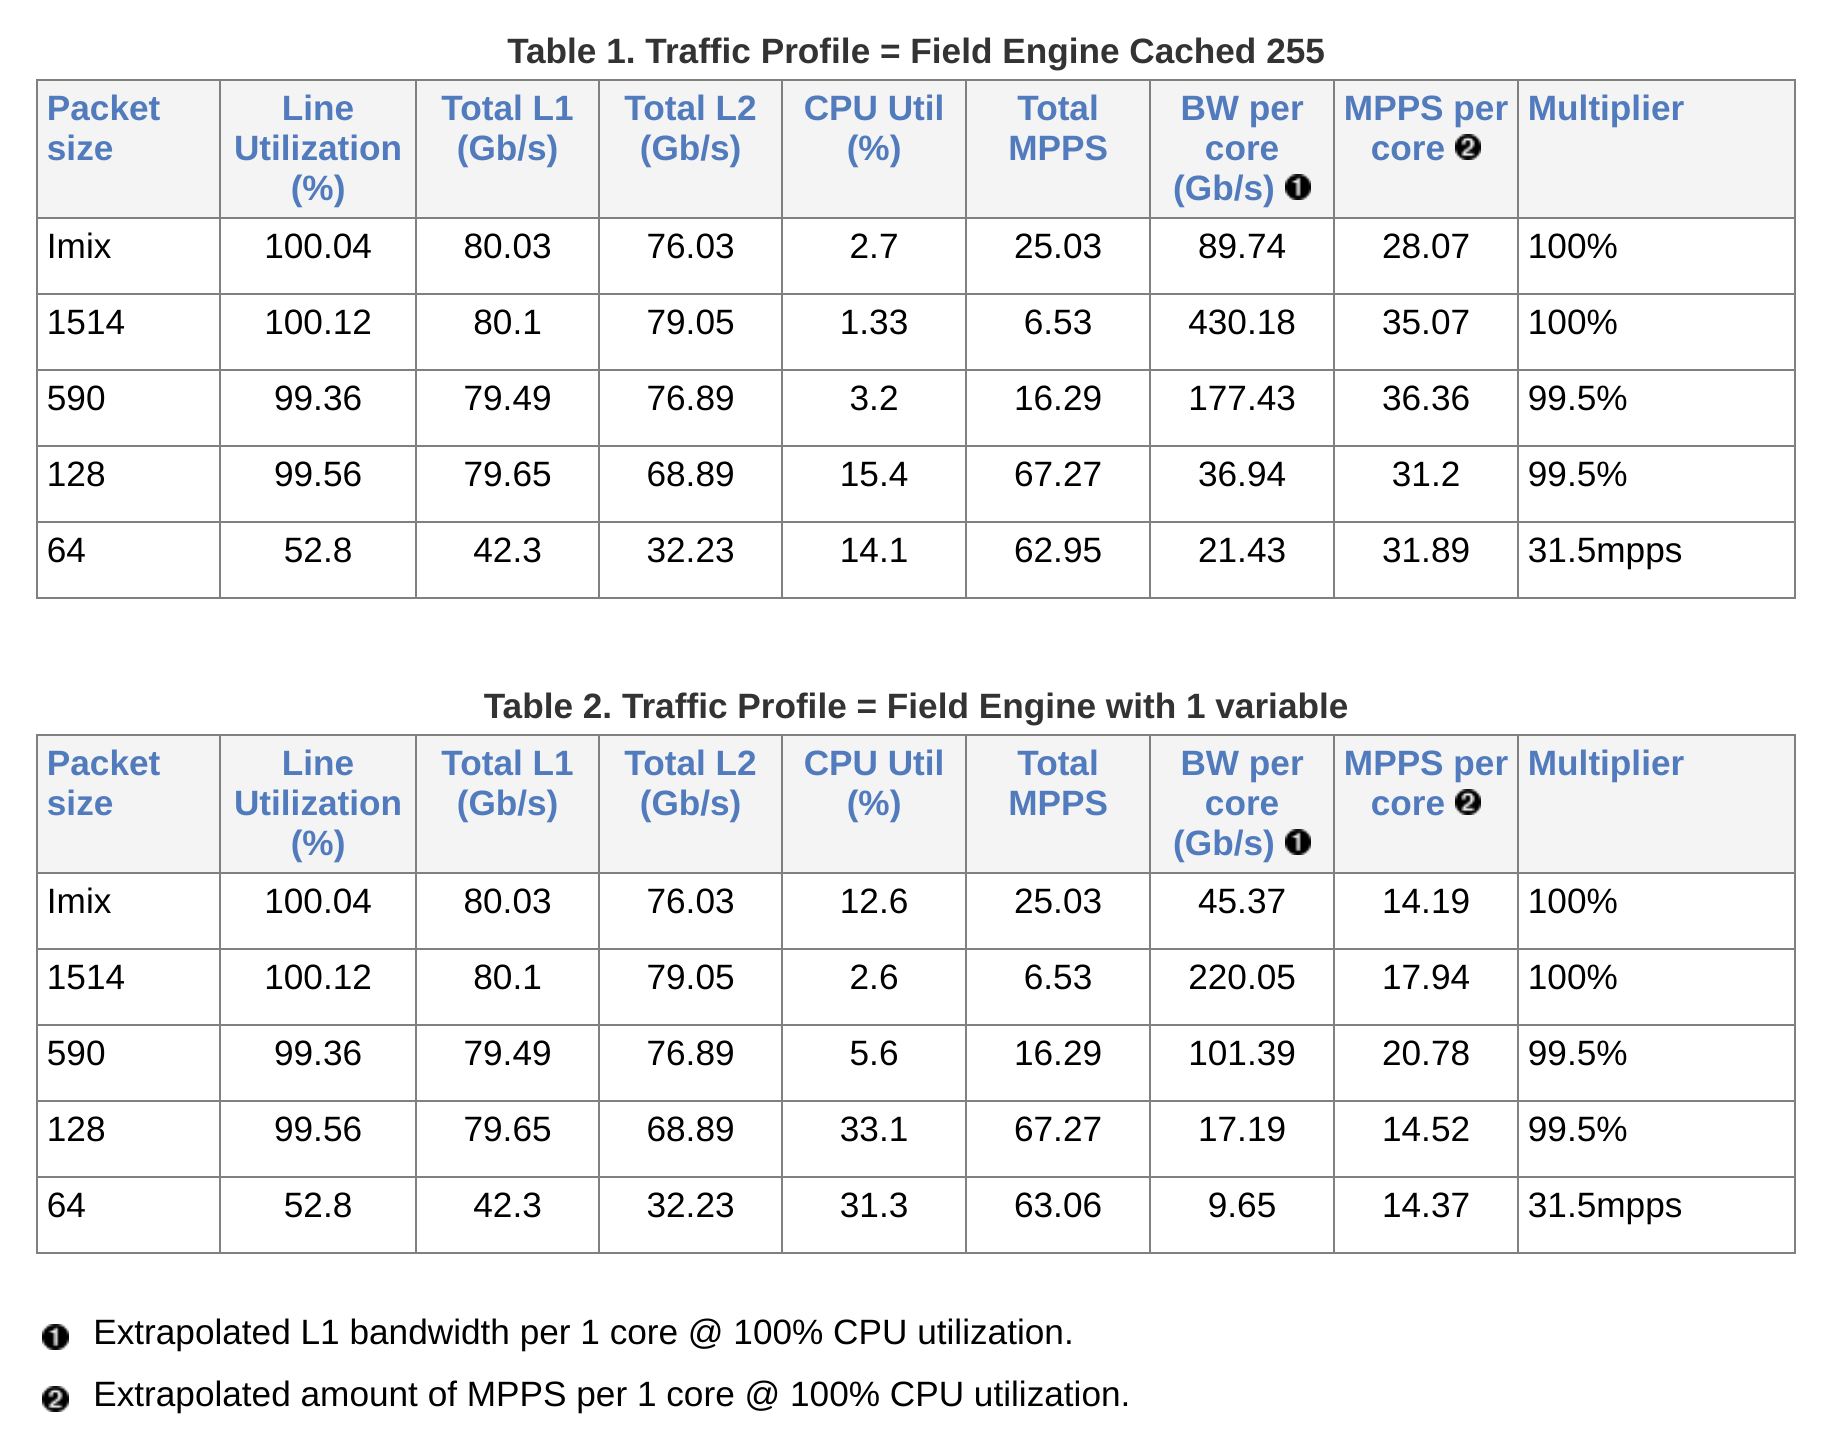
\includegraphics[width=0.4
\textwidth, center]{stl_perf.png}
\caption{Stateless performance with Intel XL710}
\label{fig:stlperf}
\end{figure}

In Figure \ref{fig:stlperf} IMIX refers to a mix of packets size see \cite{b7} with an average packet size of 364 bytes.
In case of 64B packet size the maximum L1 utilization is only 52\% due to XL710 chip limitation and not CPU/software. 

\section{Stateful mode} 

The stateful model's objective is to simulate realistic L7 applications on top of a TCP/UDP stack at high scale. A fork of a BSD TCP module running in a user space is used for this purpose. 
The scale could reach millions of flows and around 100k clients/servers up to 200gbps for one server. 
It is important to test stateful features using realistic traffic scenarios because this is the only way to estimate accurate performance metrics and identify bottlenecks in the design. 

The high level features are:

\begin{itemize}
\item Realistic traffic at high scale (flows, bandwidth, connection per second)
\item Measure latency/jitter/drop in high rate
\item Emulate L7 application, e.g. HTTP/HTTPS/Citrix- there is no need to implement the exact application.
\item TCP implementation
\item Automation Python API 
\item TCP/UDP/Application statistics (per client side/per template)
\end{itemize}

\begin{figure}[h]
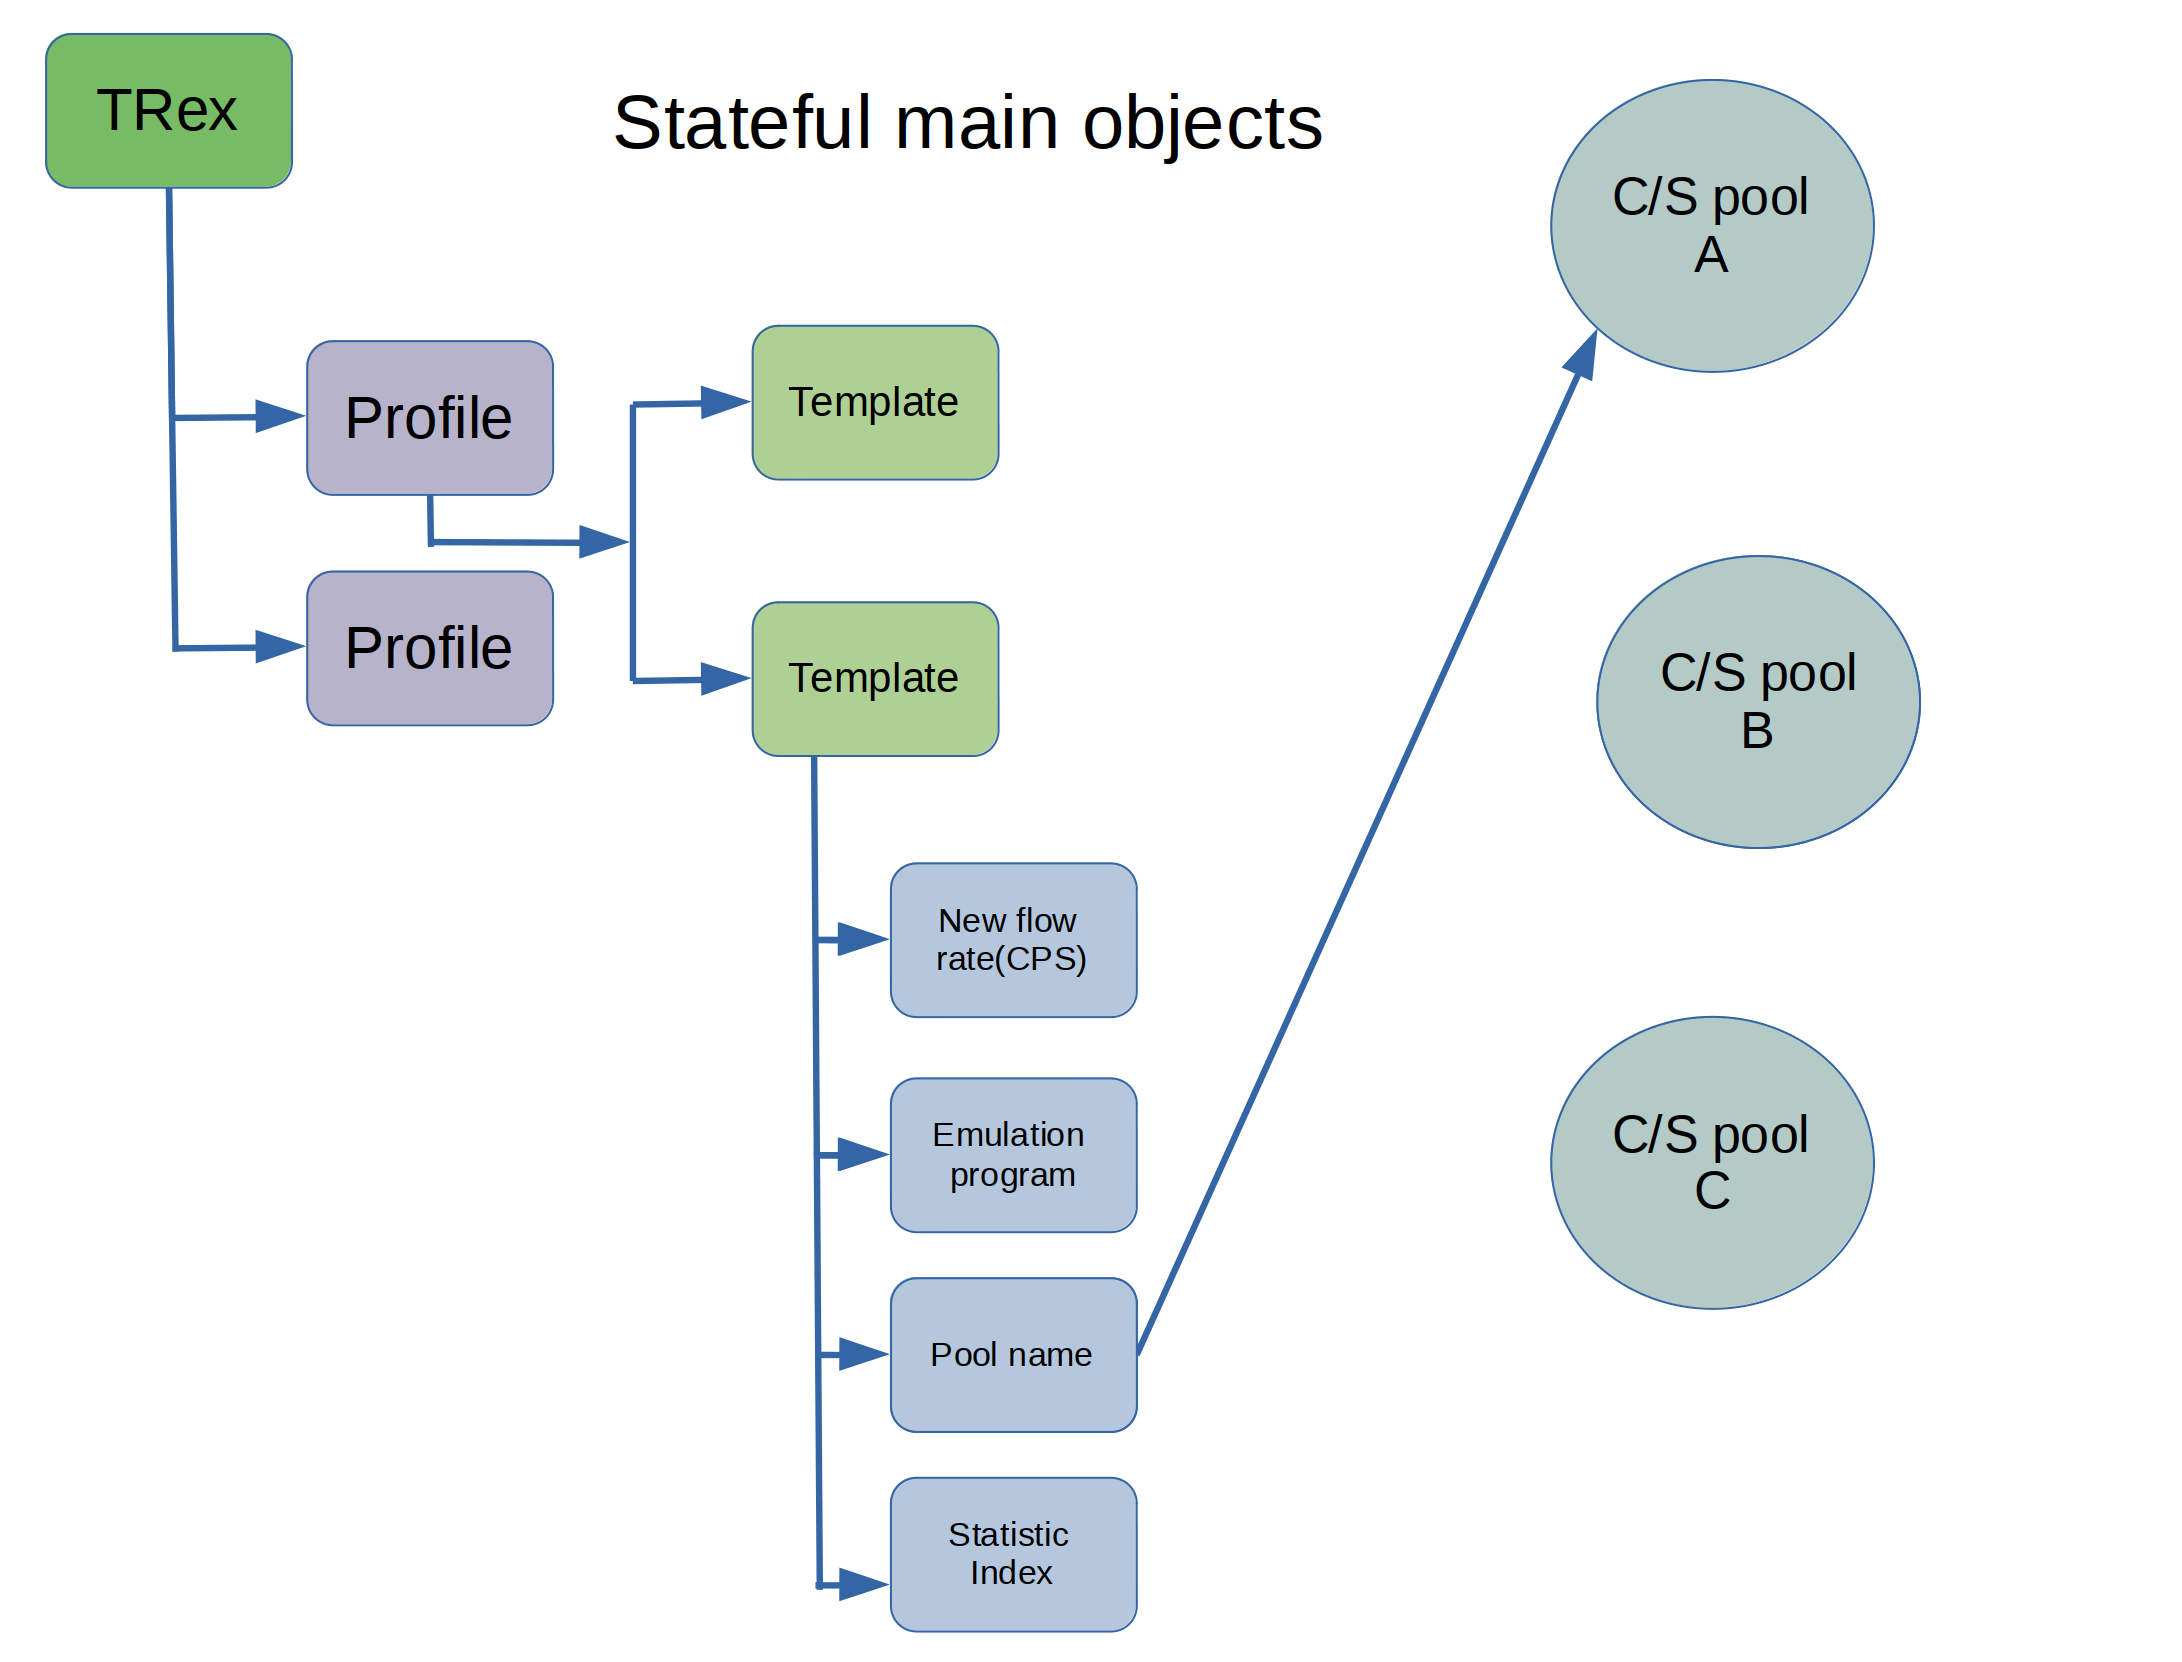
\includegraphics[width=0.45
\textwidth, center]{stateful_objects.png}
\caption{Stateful main objects}
\label{fig:astf_objects}
\end{figure}

Figure \ref{fig:astf_objects} presents the main objects in stateful mode 

Each profile includes:
\begin{itemize}
\item \textbf{Client pool}: Range of clients with a distribution model (e.g. random,seq). A profile can include a few pools.
\item \textbf{Server pool}: Range of servers, profile can include a few pools. 
\item \textbf{Template}: A model that describes an application on top of TCP/UDP. Each template could be associated with a different pool of clients/servers. The L7 data can be extracted from a pcap file and converted to an emulation program
\begin{itemize}
\item \textbf{CPS}: How many connections per second to generate for this template. 
\item \textbf{Program}: Emulation instructions to simulate the L7 application e.g. HTTP e.g. writeBuffer/readBuffer
\item \textbf{Client/Server pool name}: Associated with one of the pools
\item \textbf{Statistics pool}: The index of the TCP/UDP statistic counters pool. Good for QoS scenarios; each template could be associated with different pool of counters 
\end{itemize}
\end{itemize}

Figure \ref{fig:astf} presents the traffic generation model. 

\begin{figure}[h]
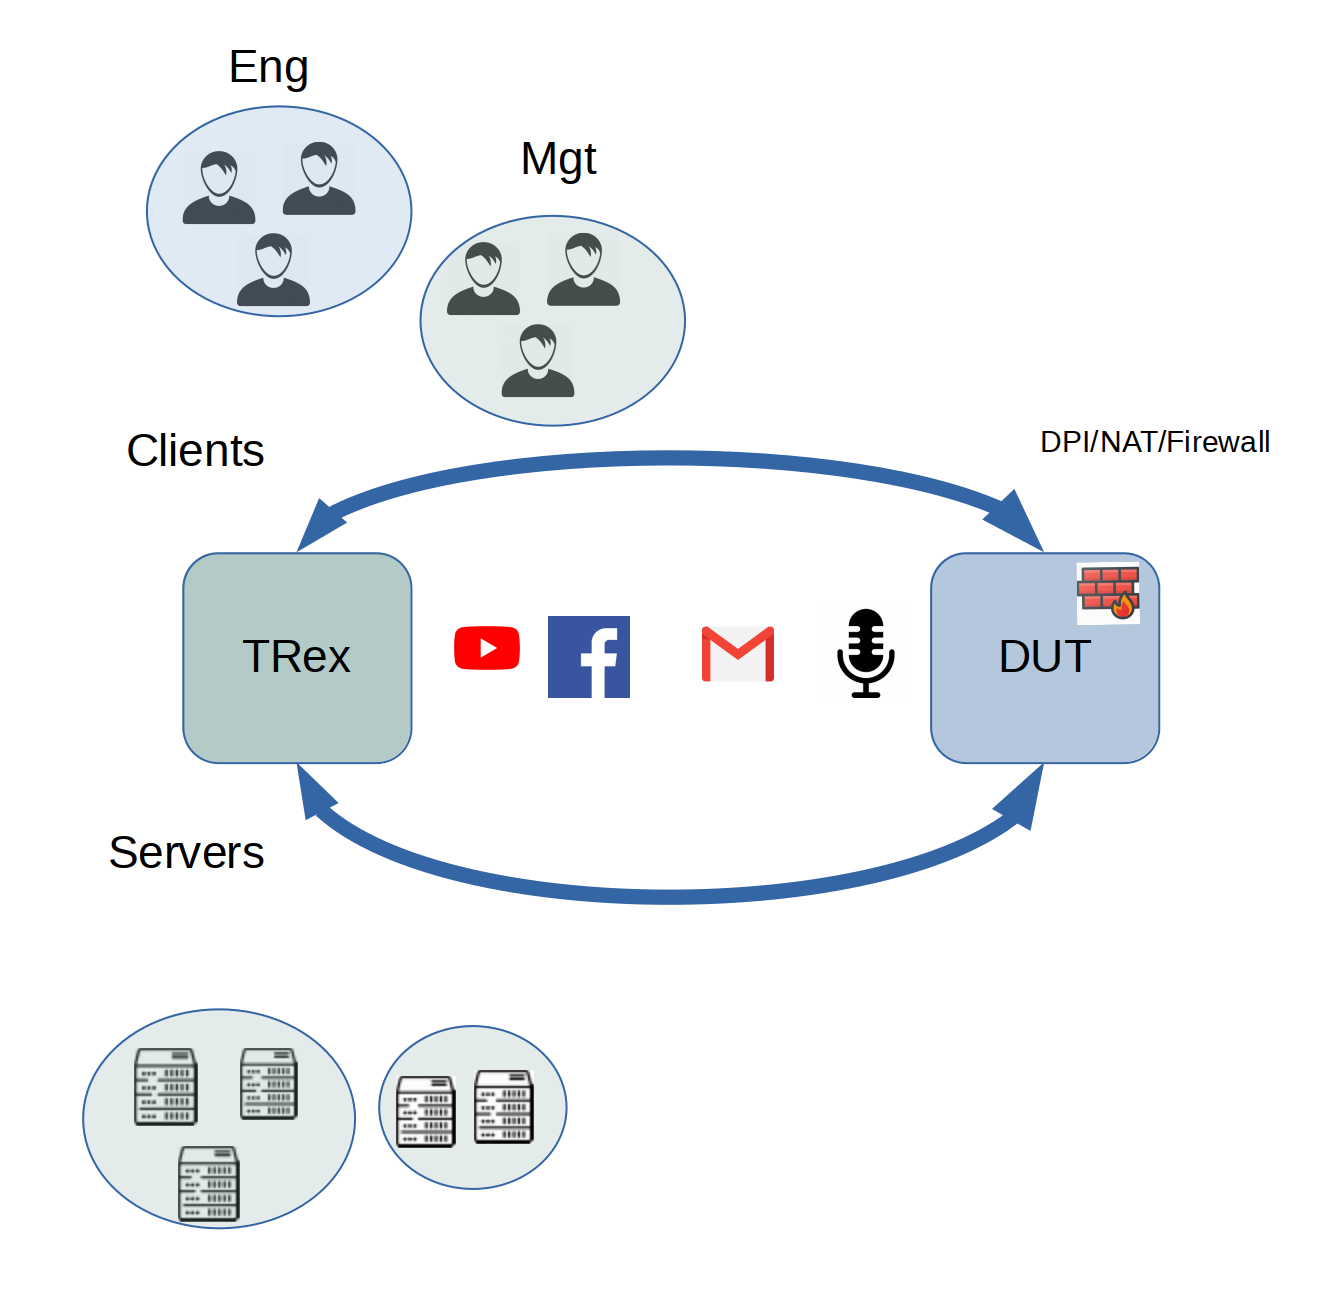
\includegraphics[width=0.3
\textwidth, center]{stateful_model.png}
\caption{Stateful model}
\label{fig:astf}
\end{figure}

In this mode, each core has its own context of TCP/UDP stack with no memory sharing and no locks. It works on top of the scheduler hierarchy shown in Figure \ref{fig:dp_schduler}.
The most significant changes to the BSD stack were:
\begin{itemize}
\item Each stack has a context per thread. No memory sharing, no locks. GRO/LRO/TSO is supported. 
\item Tx works in pool mode (it builds the packets only when required) and saves a reference to the template data. This saves three orders of magnitude of memory resource.
\end{itemize}

\begin{figure}[h]
\includegraphics[width=0.15
\textwidth, center]{t_c4.png}
\caption{Stateful stack}
\label{fig:astf_stack}
\end{figure}

Figure \ref{fig:astf_stack} shows the stack of the programmable application emulation layer. This module is responsible to simulate applications on top of the TCP/UDP stack. The program is part of a template.  
Some possible instructions are:

\begin{itemize}
\item Start write of buffer
\item Continue write
\item End Write
\item Wait for buffer/timeout
\item OnConnect/OnReset/OnClose
\end{itemize}


\subsection{Stateful Profile Example}

\begin{listing}[h]
\caption{Stateful profile}
\label{listing:7}
\begin{minted}
[
    frame=lines,
    fontsize=\scriptsize,
]
{python}
 
from trex.astf.api import *

class Prof1():
    def get_profile(self):
        # clients pool range and distribution type
        ip_gen_c = ASTFIPGenDist(
        ip_range=["16.0.0.1", "16.0.0.254"],
        distribution="seq")
        # servers pool range and distribution type
        ip_gen_s = ASTFIPGenDist(
        ip_range=["48.0.0.1", "48.0.255.254"],
        distribution="seq")
        # pool definition for both clients and servers
        ip_gen = 
        ASTFIPGen(
            glob=ASTFIPGenGlobal(ip_offset="1.0.0.0"), 
                dist_client=ip_gen_c,
                dist_server=ip_gen_s)

        # Parse the pcap file and convert to instructions 
        # cps is 1 flows/sec           
        return ASTFProfile(default_ip_gen=ip_gen,
                        cap_list=[ASTFCapInfo(
                file="../avl/delay_10_http_browsing_0.pcap"
            cps=1)
        ])
    
\end{minted}
\end{listing}

Listing \ref{listing:7} shows a simple profile with one pool of clients \texttt{(16.0.0.1-16.0.0.254)} and one pool of servers \texttt{(48.0.0.1-48.0.255.254)}. 
The pcap file is parsed and the L7 data is converted to instructions on top of the TCP stack.

\subsection{ Emulation layer instructions}

Listing \ref{listing:8} shows a simple example of low level instructions of the emulation layer. 
In this example the client sends a request and waits for the response while the server waits for the request and sends a response. 
Listing \ref{listing:client} and Listing \ref{listing:server} shows the pseudo user-space code that is executed for each flow for Listing \ref{listing:8} emulation program to better understand how it works internally. 

\begin{listing}[h]
\caption{Emulation layer instructions}
\label{listing:8}
\begin{minted}
[
    frame=lines,
    fontsize=\scriptsize,
]
{python}
 
# client side HTTP program
prog_c = ASTFProgram()
prog_c.send(http_req)
prog_c.recv(len(http_response))

# server side HTTP program
prog_s = ASTFProgram()
prog_s.recv(len(http_req))
prog_s.send(http_response)

\end{minted}
\end{listing}


\begin{listing}[h]
\caption{Client pseudo code}
\label{listing:client}
\begin{minted}
[
    frame=lines,
    fontsize=\scriptsize,
]
{python}
# for better understand how TRex works, 
# this pseudo code is the linux version of the emulation 
# layer (client side)
template = choose_template() 

src_ip,dest_ip,src_port = generate from pool of client
dst_port                = template.get_dest_port()

s = socket.socket(socket.AF_INET, 
                socket.SOCK_STREAM)

s.connect(dest_ip,dst_port)   

# program  
s.write(template.request) 
# GET /3384 HTTP/1.1
# Host: 22.0.0.3
# Connection: Keep-Alive
# User-Agent: Mozilla/4.0
# Accept: */*
# Accept-Language: en-us
# Accept-Encoding: gzip, deflate, compress

s.read(template.request_size) 
#HTTP/1.1 200 OK
#Server: Microsoft-IIS/6.0
#Content-Type: text/html
#Content-Length: 32000
# body ..


s.close();

\end{minted}
\end{listing}


\begin{listing}[h]
\caption{Server pseudo code}
\label{listing:server}
\begin{minted}
[
    frame=lines,
    fontsize=\scriptsize,
]
{python}
# for better understand how TRex works, 
# this pseudo code is the linux version of the emulation 
# layer (server side)
# if this is SYN for flow that already exist, 
let TCP handle it

if ( flow_table.lookup(pkt) == False ) :
    # first SYN in the right direction with no flow
    compare (pkt.src_ip/dst_ip to the generator ranges) 
    # check that it is in the range or 
    valid server IP (src_ip,dest_ip)
    #get template for the dest_port
    template= lookup_template(pkt.dest_port) 

    # create a socket for TCP server
    s = socket.socket(socket.AF_INET, socket.SOCK_STREAM)               1

    # bind to the port
    s.bind(pkt.dst_ip, pkt.dst_port)

    s.listen(1)
    #program of the template                                            2
    s.read(template.request_size)   

    GET /3384 HTTP/1.1
    Host: 22.0.0.3
    Connection: Keep-Alive
    User-Agent: Mozilla/4.0 ..
    Accept: */*
    Accept-Language: en-us
    Accept-Encoding: gzip, deflate, compress


    s.write(template.response)   
    #HTTP/1.1 200 OK
    #Server: Microsoft-IIS/6.0
    #Content-Type: text/html
    #Content-Length: 32000
    # body ..

    s.close()
\end{minted}
\end{listing}




\subsection{Automation example}

Listing \ref{listing:10} shows an example of a Python script to automate a stateful profile and read the port and the TCP statistics.

\begin{listing}[h]
\caption{Stateful automation example}
\label{listing:10}
\begin{minted}
[
    frame=lines,
    fontsize=\scriptsize,
]
{python}
 
c = ASTFClient(server = server)

c.connect()

try:
    c.reset()

    c.load_profile(profile_path)

    c.clear_stats()

    c.start(mult = mult, 
        duration = duration, 
        nc = True)

    c.wait_on_traffic()

    stats = c.get_stats()

    pprint.pprint(stats)

    if c.get_warnings():
        for w in c.get_warnings():
            print(w)


except TRexError as e:
    print(e)

except AssertionError as e:
    print(e)

finally:
    c.disconnect()
\end{minted}
\end{listing}

\section{Stateful optimization}

\begin{figure}[h]
\includegraphics[width=0.15
\textwidth, center]{t_c5.png}
\caption{One Flow Tx Ring}
\label{fig:tx_ring}
\end{figure}

Most TCP stacks have an API that allow the user to provide a buffer (write operation). 
The TCP module stores the buffer until the data is acknowledged by the remote side. 
With big TCP windows (required with high RTT) and many flows this could create a memory scale issue. 
Figure \ref{fig:tx_ring} shows one TCP flow Tx queue and Figure \ref{fig:rx_ring} shows the Rx side of the same flow. For 1M active flows with a 64K Tx buffer 
the worst case memory requirement is $1M \cdot 64K \cdot  mbufs  = 128GB$
The mbuf resource is expensive and needs to be allocated ahead of time (because it is shared with the NIC and translation virtual/physical need to be known). 
The chosen solution for this problem is to change the API to be a poll API, 
meaning the TCP Tx queue will just save a reference to the constant traffic and offset. The packets will be assembled with a reference to a constant mbufs only when packets need to be sent (lazy). 
Now because most of the traffic is almost constant in traffic generation cases (per template) and known ahead of time it was possible to implement and save most of the memory.
The same idea happens in the Rx side with reassembly. \footnote{This will not work for TLS streams}

\begin{figure}[h]
\includegraphics[width=0.15
\textwidth, center]{t_c6.png}
\caption{One Flow Rx Ring}
\label{fig:rx_ring}
\end{figure}


\section{Benchmark  TRex vs Linux kernel}

To evaluate the performance and memory scale of TRex and compare it against standard Linux tools the following was done: 
Linux \texttt{nginx} as a server were compared to TRex for stressing a device under test.

\begin{figure}[h]
\includegraphics[width=0.3
\textwidth, center]{nginx_setup1.png}
\caption{TRex,NGINX server Performance Testing}
\label{fig:trex_nginx}
\end{figure}

The benchmark setup was designed to take a popular event-driven Linux server application and to test using a TRex client. 
TRex client requests the pages. Figure \ref{fig:trex_nginx} shows the topology in this case. TRex is in a different server connected to the \texttt{nginx} server with 10gbps fiber. 
\texttt{nginx} is installed on another server. TRex generates requests using one DP core/thread and exercises the whole 16 cores of the \texttt{nginx}/Linux server. 
After some trial and error, it was determined that it is more difficult to separate Linux kernel/IRQ contexts events from user space process CPU, 
so it was chosen to give the \texttt{nginx} all the server resources, and monitor to determine the limiting factor.
The objective is to create a new TCP flow for each HTTP request/response session instead of keeping the same TCP flow opened and just generate a new request/response. 
This might be the main difference between \texttt{nginx}'s benchmark configuration and this document's configuration. 

\begin{figure}[h]
\includegraphics[width=0.3
\textwidth, center]{nginx_setup2.png}
\caption{TRex Client Server}
\label{fig:trex_vs_trex}
\end{figure}

To provide a baseline benchmark, the \texttt{nginx} server was replaced with a TRex server with one DP core, using an XL710 NIC (40Gb). 
see Figure \ref{fig:trex_vs_trex}. In this case there was need for a faster NIC so XL710 NIC was used (40gbps) instead of X710 (10gbps)

\subsection{Benchmark traffic profile}

Typically, web servers are tested with a constant number of active flows that are opened ahead of time. 
In the \texttt{nginx} benchmark blog, only 50 TCP constant connections are used with many requests/responses 
For each TCP connection see here \cite{b6}. In our traffic generation use case, each HTTP request/response (for each new TCP connection) requires opening a \textbf{new} TCP connection. 
A simple HTTP flow with a request of 100B and a response of 32KB (about 32 packets/flow with initwnd=2) was used.
We used this profile because it is part of our EMIX profile. 

\subsection{Benchmark Limitations}

The comparison is not perfect, as TRex merely emulates HTTP traffic. 
It is not a real-world web server or HTTP client. For example, currently the TRex client does not parse the HTTP response for the Length field. 
TRex simply waits for a specific data size (32KB) over TCP. However the TCP layer is a fully featured TCP (e.g. delay-ack/Retransmission/Reassembly/timers) . 
The benchmark's objective is to compare traffic generation capabilities for stressing network gears and not to replace \texttt{nginx} servers. 

\subsection{Benchmark results}

Comparing 1 DP core running TRex to \texttt{nginx} running on 16 cores with a kernel that can interrupt any \texttt{nginx} process with IRQ. Figure \ref{fig:trex_nginx_r1} shows the performance of one DP TRex. \texttt{m} stands for multiplier of the baseline profile. 
It can scale to about 25Gb/sec of download of HTTP (total of 3MPPS/90KCPS/60k active flows for one core).

\begin{figure}[h]
\includegraphics[width=0.5
\textwidth, center]{nginx_result_trex1.png}
\caption{TRex 1 DP core}
\label{fig:trex_nginx_r1}
\end{figure}

\begin{figure}[h]
\includegraphics[width=0.5
\textwidth, center]{nginx_result_linux1.png}
\caption{NGINX 16 cores}
\label{fig:trex_nginx_r2}
\end{figure}

\texttt{nginx} cannot handle more than 20K new flows/sec, due to the kernel TCP software IRQ interrupts processing. 
The limitation is the kernel and not \texttt{nginx}'s user space process.
With more NICs and optimized distribution, the number of flows could be increased times two, but not more than that. 
The total number of packets was approximately 600KPPS (Tx+Rx). The number of active flows was 12K.

TRex with one core could scale to about 25Gb/sec, 3MPPS of the same HTTP profile.
The main issue with \texttt{nginx} and Linux setup is the tunning (this might be improved with more sophisticated tunning). 
It is very hard to let the hardware utilize the full server resource (half of the server was idle in this case and still experienced a lot of drop). 
TRex is not perfect too, we couldn't reach 100\% CPU utilization without a drop (CPU was 84\%). To achieve 100gbps with this profile on the server side requires ~4 cores for TRex, vs. 20x16 cores for \texttt{nginx} servers. 
TRex is faster by a factor of \textbf{80}. In this implementation, each flow requires approximately 1K bytes of memory (regardless of Tx/Rx rings because of TRex architecture). 
In the kernel, with a real-world server, TRex optimization can't be applied and each TCP connection must save memory in Tx/Rx rings.
For about 5Gb/sec traffic with this profile, approximately 10GB of memory was required (both \texttt{nginx} and Kernel). For 100Gb/sec traffic, approximately 200GB is required (extrapolation)  With a TRex optimized implementation, approximately 100MB is required. 
TRex thus provides an improvement by a factor or \textbf{2000} in the use of memory resources.

\section{Routing protocol using BIRD}

Bird Internet Routing Daemon \cite{b4} is a project aimed to develop a fully functional Linux dynamic IP routing daemon for BGP/OSPF/RIP and more. 
It was integrated into TRex to run alongside in order to exploit it’s features together with Python automation API using Linux network namespace and veth. 
In this case the Linux TCP stack is used (e.g. BGP) and packets from the veth is moved from/to to the physical ports. 
Figure \ref{fig:bird} shows the integration with TRex server. The pyBird server is a daemon that receives JSON-RPC2 over ZMQ RPC commands from one side and interact with BIRD daemon using ssh/text protocol. 
The BIRD automation API interacts with both BIRD and TRex to set the right filters and configure the veth/. Using the API, one can push 1M of BGP routes in a few seconds to the DUT.

\begin{figure}[h]
\includegraphics[width=0.5
\textwidth, center]{trex_bird_general_scheme.png}
\caption{BIRD TRex integration}
\label{fig:bird}
\end{figure}

\begin{figure}[h]
    \includegraphics[width=0.5
    \textwidth, center]{TRex_Bird_General_Scheme_With_ips.png}
    \caption{BIRD Simple Example}
    \label{fig:bird_example}
\end{figure}
  
    
Figure \ref{fig:bird_example} show a simple example of configuration with 2 ports. BIRD has 2 veth's in the same subnet of TRex ports. 
Listing \ref{listing:bird} shows a sample profile to push 11 BGP routes 42.42.42.0-10/32 via 1.1.1.3



\begin{listing}[h]
\caption{BIRD configuration}
\label{listing:bird}
\begin{minted}
[
    frame=lines,
    fontsize=\scriptsize,
]
{python}

router id 100.100.100.100;

protocol device {
    scan time 1;
}

protocol bgp my_bgp1 {
    # put your local ip and as number here
    local 1.1.1.3 as 65000;  
    # put your dut ip and as number here
    neighbor 1.1.1.1 as 65000;  
    ipv4 {
        import all;
        export all;
    };
}

# using a second interface
protocol bgp my_bgp2 {
    # same for the second interface
    local 1.1.2.3 as 65000;  
    neighbor 1.1.2.1 as 65000;
    ipv4 {
        import all;
        export all;
    };
}

protocol static {
    ipv4 {
        import all;
        export all;
    };

    route 42.42.42.0/32 via 1.1.1.3;
    route 42.42.42.1/32 via 1.1.1.3;
    route 42.42.42.2/32 via 1.1.1.3;
    route 42.42.42.3/32 via 1.1.1.3;
    route 42.42.42.4/32 via 1.1.1.3;
    route 42.42.42.5/32 via 1.1.1.3;
    route 42.42.42.6/32 via 1.1.1.3;
    route 42.42.42.7/32 via 1.1.1.3;
    route 42.42.42.8/32 via 1.1.1.3;
    route 42.42.42.9/32 via 1.1.1.3;
    route 42.42.42.10/32 via 1.1.1.3;
}

\end{minted}
\end{listing}

\section{Acknowledgments}
This project was incubated inside Cisco Systems with a small team: Lior Katzri, 
Itay Marom, Ido Barnea and Yaroslav Brustinov. Today there are many contributers but I would like to mention Gwangmoon Kim team from Ericsson for the discussions, suggestions 
and contribution of many complex features. 

\newpage

\begin{thebibliography}{00}
\bibitem{b1} Cisco systems: ``TRex realistic traffic generator'',\\\texttt{https://trex-tgn.cisco.com/trex/doc/}
\bibitem{b2} Cisco systems, ``TRex Stateless'',,\\\texttt{https://trex-tgn.cisco.com/trex/doc/trex\_stateless.html}
\bibitem{b3} Cisco systems, ``TRex Stateful ASTF'',,\\\texttt{https://trex-tgn.cisco.com/trex/doc/trex\_astf.html}
\bibitem{b4} BIRD, Faculty of Math and Physics, Charles University Prague \\\texttt{https://bird.network.cz/}
\bibitem{b5} Cisco systems, ``TRex STL benchmark'',,\\\texttt{https://trex-tgn.cisco.com/trex/doc/trex\_stateless\_bench.html}
\bibitem{b6} NGINX performance  \\\texttt{https://www.nginx.com/blog/testing-the-performance-of-nginx-and-nginx-plus-web-servers/}
\bibitem{b7} IMIX  \\\texttt{https://en.wikipedia.org/wiki/Internet\_Mix}
\end{thebibliography}

\end{document}
